\documentclass[border=1mm]{standalone}
\usepackage[T1]{fontenc}
\usepackage[scaled=0.92]{helvet}
\renewcommand\familydefault{\sfdefault}
\usepackage{amssymb}
\usepackage{tikz}
\usetikzlibrary{arrows.meta,calc,shapes.geometric}
% ---- shared style (methodology figures) ----
\definecolor{mA}{HTML}{1B7F79}\definecolor{mAl}{HTML}{E4F2F0}
\definecolor{mB}{HTML}{2F5F98}\definecolor{mBl}{HTML}{E7EEF7}
\definecolor{mC}{HTML}{B85A16}\definecolor{mCl}{HTML}{FBEEDF}
\definecolor{ink}{HTML}{262626}\definecolor{mute}{HTML}{6B6B6B}
\definecolor{grey}{HTML}{8C8C8C}\definecolor{greyl}{HTML}{EFEFEF}
% pathway colours: ECM, TGF-beta, stellate, inflammation, apoptosis/stress, hepatocyte
\definecolor{pw0}{HTML}{B85A16}\definecolor{pw1}{HTML}{D9A21B}\definecolor{pw2}{HTML}{8A5BA6}
\definecolor{pw3}{HTML}{C2413B}\definecolor{pw4}{HTML}{6E8B3D}\definecolor{pw5}{HTML}{2F5F98}
\newcommand\fs{\fontsize{7}{8.4}\selectfont}
\newcommand\fss{\fontsize{6.3}{7.5}\selectfont}
\newcommand\fsx{\fontsize{5.8}{6.8}\selectfont}
\newcommand\fsh{\fontsize{7.6}{9}\selectfont\bfseries}
\newcommand\fsn{\fontsize{9}{10}\selectfont\bfseries}
\hyphenpenalty=10000 \exhyphenpenalty=10000
\tikzset{
  >={Stealth[length=2mm,width=1.6mm]},
  flow/.style={->,line width=0.8pt,draw=ink!70},
  thin/.style={->,line width=0.5pt,draw=ink!60},
  gedge/.style={draw=black!22,line width=0.25pt},
  gnode/.style={circle,draw=white,line width=0.25pt,inner sep=0pt,minimum size=1.45mm},
  ttl/.style={anchor=west,font=\fsh},
}
% cylinder: \cyl{colour}{x centre}{base y}{height}{width}
\newcommand\cyl[5]{%
  \filldraw[fill=#1!35,draw=#1,line width=0.5pt] ({#2-#5/2},{#3+#4}) -- ({#2-#5/2},#3) arc[start angle=180,end angle=360,x radius=#5/2,y radius=0.9] -- ({#2+#5/2},{#3+#4});
  \filldraw[fill=#1!12,draw=#1,line width=0.5pt] (#2,{#3+#4}) ellipse[x radius=#5/2,y radius=0.9];}
% numbered module badge
\newcommand\badge[3]{\node[circle,fill=#1,text=white,inner sep=0pt,minimum size=4.6mm,font=\fss\bfseries] at #2 {#3};}
\newcommand\bx[3]{% x, median y, colour : one cohort's expression distribution
  \draw[#3,line width=0.4pt] (#1,#2-3.6)--(#1,#2+3.6);
  \filldraw[fill=#3!30,draw=#3,line width=0.4pt] (#1-0.9,#2-1.8) rectangle (#1+0.9,#2+1.8);
  \draw[#3,line width=0.7pt] (#1-0.9,#2)--(#1+0.9,#2);}
\newcommand\lk[1]{\node[diamond,fill=mC,inner sep=0pt,minimum size=2.3mm] at #1 {};}
\begin{document}
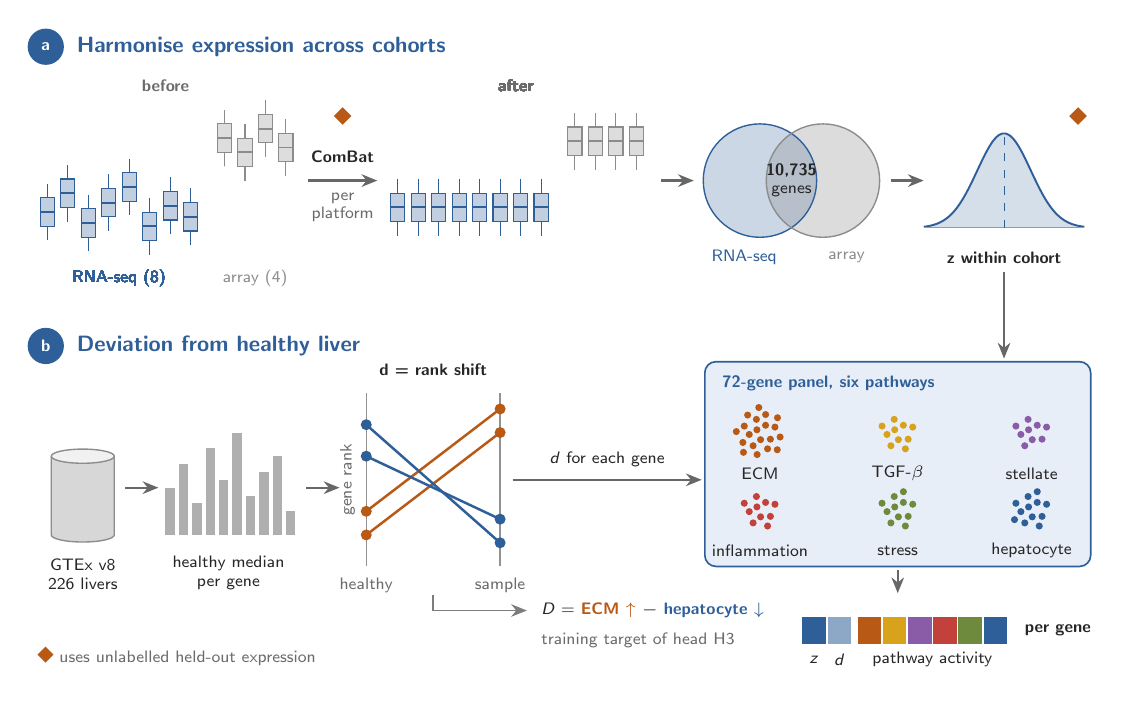
\begin{tikzpicture}[x=1mm,y=1mm,font=\fs,text=ink]
% =============== row 1: harmonise expression ===============
\badge{mB}{(2.3,79)}{a}
\node[ttl,text=mB] at (5,79) {Harmonise expression across cohorts};
% before
\foreach \m [count=\i from 0] in {58,60.4,56.6,59.2,61.2,56.2,58.8,57.4} \bx{2.5+\i*2.6}{\m}{mB}
\foreach \m [count=\i from 0] in {67.4,65.6,68.6,66.2} \bx{25+\i*2.6}{\m}{grey}
\node[font=\fsx,text=mB] at (11.6,49.6) {RNA-seq (8)};
\node[font=\fsx,text=grey] at (28.9,49.6) {array (4)};
\node[font=\fss\bfseries,text=mute] at (17.5,74) {before};
% ComBat arrow
\draw[flow] (35.6,62)--(44.4,62);
\node[font=\fss\bfseries,anchor=south] at (40,63) {ComBat};
\node[font=\fsx,text=mute,align=center] at (40,58.6) {per\\platform};
\lk{(40,70.2)}
% after
\foreach \i in {0,...,7} \bx{47+\i*2.6}{58.6}{mB}
\foreach \i in {0,...,3} \bx{69.5+\i*2.6}{67}{grey}
\node[font=\fss\bfseries,text=mute] at (62,74) {after};
% intersect (Venn)
\draw[flow] (80.4,62)--(84.6,62);
\fill[mB,opacity=0.25] (93,62) circle (7.2);
\fill[grey,opacity=0.3] (101,62) circle (7.2);
\draw[mB,line width=0.5pt] (93,62) circle (7.2); \draw[grey,line width=0.5pt] (101,62) circle (7.2);
\node[font=\fss\bfseries,align=center] at (97,62) {10,735\\[-1pt]{\fsx\mdseries genes}};
\node[font=\fsx,text=mB] at (91,52.2) {RNA-seq};
\node[font=\fsx,text=grey] at (104,52.2) {array};
% within-cohort scaling
\draw[flow] (109.6,62)--(113.8,62);
\fill[mB!20] plot[domain=-3:3,samples=50,smooth] ({124+\x*3.4},{56+12*exp(-\x*\x/2)}) -- cycle;
\draw[mB,line width=0.7pt] plot[domain=-3:3,samples=50,smooth] ({124+\x*3.4},{56+12*exp(-\x*\x/2)});
\draw[mB!60,line width=0.4pt] (113.8,56)--(134.2,56);
\draw[mB,dashed,line width=0.4pt] (124,56)--(124,68);
\node[font=\fss\bfseries] at (124,52.2) {\textit{z} within cohort};
\lk{(133.4,70.2)}
% =============== row 2: healthy reference ===============
\badge{mB}{(2.3,41)}{b}
\node[ttl,text=mB] at (5,41) {Deviation from healthy liver};
\cyl{grey}{7}{17}{10}{8}
\node[font=\fsx,align=center] at (7,12) {GTEx v8\\226 livers};
\draw[flow] (12.4,23)--(16.6,23);
% healthy median profile (sparkline)
\foreach \h [count=\i from 0] in {6,9,4,11,7,13,5,8,10,3} \fill[grey!70] (17.5+\i*1.7,17) rectangle ++(1.2,\h);
\node[font=\fsx,align=center] at (25.5,12.2) {healthy median\\per gene};
\draw[flow] (35.4,23)--(39.6,23);
% slopegraph: rank in healthy profile vs rank in one sample
\draw[ink!50,line width=0.5pt] (43,13)--(43,35); \draw[ink!50,line width=0.5pt] (60,13)--(60,35);
\node[font=\fsx,text=mute] at (43,10.6) {healthy};
\node[font=\fsx,text=mute] at (60,10.6) {sample};
\node[font=\fsx,text=mute,rotate=90] at (40.6,24) {gene rank};
\foreach \a/\b in {17/30,20/33} {\draw[pw0,line width=0.9pt] (43,\a)--(60,\b); \fill[pw0] (43,\a) circle (0.7); \fill[pw0] (60,\b) circle (0.7);}
\foreach \a/\b in {31/16,27/19} {\draw[pw5,line width=0.9pt] (43,\a)--(60,\b); \fill[pw5] (43,\a) circle (0.7); \fill[pw5] (60,\b) circle (0.7);}
\node[font=\fss\bfseries] at (51.5,38) {\textit{d} = rank shift};
% directional target
\node[anchor=west,font=\fss] at (64,7.4) {\textit{D} = \textcolor{pw0}{\textbf{ECM $\uparrow$}} $-$ \textcolor{pw5}{\textbf{hepatocyte $\downarrow$}}};
\node[anchor=west,font=\fsx,text=mute] at (64,3.6) {training target of head H3};
\draw[thin] (51.5,9.4) |- (63.4,7.4);
% d into the panel
\draw[flow] (61.6,24)--(85.6,24);
\node[anchor=south,font=\fss] at (73.6,24.4) {\textit{d} for each gene};
% =============== 72-gene panel ===============
\draw[flow] (124,50.4)--(124,39.4);
\filldraw[fill=mBl,draw=mB,line width=0.6pt,rounded corners=1.4mm] (86,13) rectangle (135,39);
\node[anchor=north west,font=\fss\bfseries,text=mB] at (87,38.4) {72-gene panel, six pathways};
\newcommand\clus[5]{% x, y, count, colour, name
  \foreach \k in {1,...,#3} {\pgfmathsetmacro\r{0.74*sqrt(\k-0.5)} \pgfmathsetmacro\t{\k*137.508}
     \fill[#4] ({#1+\r*cos(\t)},{#2+0.6+\r*sin(\t)}) circle (0.45);}
  \node[font=\fsx] at (#1,#2-4.6) {#5};}
\clus{93}{29.4}{20}{pw0}{ECM}
\clus{110.5}{29.4}{10}{pw1}{TGF-$\beta$}
\clus{127.5}{29.4}{9}{pw2}{stellate}
\clus{93}{19.6}{10}{pw3}{inflammation}
\clus{110.5}{19.6}{11}{pw4}{stress}
\clus{127.5}{19.6}{12}{pw5}{hepatocyte}
% output strip: 8 sample-specific features per gene
\draw[flow] (110.5,12.6)--(110.5,9.6);
\fill[mB] (98.4,3.2) rectangle ++(3,3.4); \fill[mB!55] (101.6,3.2) rectangle ++(3,3.4);
\foreach \c [count=\i from 0] in {pw0,pw1,pw2,pw3,pw4,pw5} \fill[\c] (105.4+\i*3.2,3.2) rectangle ++(3,3.4);
\node[font=\fsx] at (99.9,1.2) {\textit{z}}; \node[font=\fsx] at (103.1,1.2) {\textit{d}};
\node[font=\fsx] at (114.9,1.2) {pathway activity};
\node[anchor=west,font=\fss\bfseries] at (125.4,4.9) {per gene};
% legend
\node[anchor=west,font=\fsx,text=mute] at (0,1.6) {\tikz\node[diamond,fill=mC,inner sep=0pt,minimum size=2.1mm]{}; uses unlabelled held-out expression};
\end{tikzpicture}
\end{document}
